% Fact sheet for MATH 300, for Fall 2014.
\documentclass{article}[12pt]

% useful packages
\usepackage{fullpage}
\usepackage{amsmath,amssymb,amsthm,amsfonts}
\usepackage{graphicx}
\usepackage{enumerate}
\usepackage{algorithm,algorithmic}
\usepackage{xcolor}
\usepackage{bbm}
\usepackage{url}
\usepackage{caption,subcaption}

% theorem type environments
\newtheorem{thm}{Theorem}
\newtheorem{prop}{Proposition}
\newtheorem{lemma}{Lemma}
\newtheorem{cor}{Corollary}
\newtheorem{defn}{Definition}
\newtheorem{assump}{Assumption}
\newtheorem{example}{Example}
\newtheorem{conjecture}{Conjecture}

% frequently used symbols
\newcommand{\bE}{\mathbb{E}}
\newcommand{\bP}{\mathbb{P}}
\newcommand{\bQ}{\mathbb{Q}}
\newcommand{\bR}{\mathbb{R}}
\newcommand{\bS}{\mathbb{S}}
\newcommand{\bN}{\mathbb{N}}
\newcommand{\bZ}{\mathbb{Z}}
\newcommand{\sC}{{\mathcal C}} 
\newcommand{\sD}{{\mathcal D}} 
\newcommand{\sE}{{\mathcal E}} 
\newcommand{\sF}{{\mathcal F}} 
\newcommand{\sL}{{\mathcal L}} 
\newcommand{\sH}{{\mathcal H}} 
\newcommand{\sN}{{\mathcal N}} 
\newcommand{\sO}{{\mathcal O}} 
\newcommand{\sP}{{\mathcal P}} 
\newcommand{\sR}{{\mathcal R}} 
\newcommand{\sS}{{\mathcal S}}
\newcommand{\sU}{{\mathcal U}} 
\newcommand{\sX}{{\mathcal X}} 
\newcommand{\sY}{{\mathcal Y}} 
\newcommand{\sZ}{{\mathcal Z}}

% operators
\newcommand{\sign}{\mathop{\mathrm{sign}}}
\newcommand{\supp}{\mathop{\mathrm{supp}}} % support
\newcommand{\argmin}{\operatornamewithlimits{arg\ min}}
\newcommand{\argmax}{\operatornamewithlimits{arg\ max}}
\newcommand{\dist}{\operatorname{dist}}
\newcommand{\tr}{\text{tr}}
\newcommand{\vecop}{\text{vec}}
\newcommand{\st}{\operatorname{s.t.}}
\newcommand{\cut}{\setminus}
\newcommand{\ra}{\rightarrow}
\newcommand{\ind}[1]{\mathbbm{1}\left\{#1\right\}} 
\newcommand{\given}{\ | \ }

% grouping operators
\newcommand{\brac}[1]{\left[#1\right]}
\newcommand{\set}[1]{\left\{#1\right\}}
\newcommand{\abs}[1]{\left\lvert #1 \right\rvert}
\newcommand{\paren}[1]{\left(#1\right)}
\newcommand{\norm}[1]{\left\|#1\right\|}
\newcommand{\ip}[2]{\left\langle #1,#2 \right\rangle}

% code commands
\newcommand{\matlab}{\textsc{Matlab }}
\newcommand{\algname}[1]{\textnormal{\textsc{#1}}}

\graphicspath{{./img/}}

% header command
\newcommand{\homework}[4]{
    \pagestyle{myheadings}
    \thispagestyle{plain}
    \newpage
    \setcounter{page}{1}
    \setlength{\headsep}{10mm}
    \noindent
    \begin{center}
    \framebox{
        \vbox{\vspace{2mm}
            \hbox to 6.28in { {\bf STAT 672: Statistical Learning II
            \hfill Winter 2020} }
        \vspace{4mm}
        \hbox to 6.28in { {\Large \hfill Homework #1 \hfill} }
        \vspace{2mm}
        \hbox to 6.28in { \Large \hfill Due: #2 \hfill }
        \vspace{2mm}
        \hbox to 6.28in { {\it Student Name: #3} \hfill {\it Professor Name: #4}}
        \vspace{2mm}}
   }
   \end{center}
   \markboth{Homework #1}{Homework #1}
   \vspace*{4mm}
}

\begin{document}
\homework{4}{February 19th, 2020}{Ethan Lew}{Bruno Jedynak}
\section{Multivariate Normal random Vectors (MVN)}

Let $X \sim MVN(\mu,\Sigma)$. Let $\lambda_1 \geq \ldots \lambda_m > 0 = \lambda_{m+1} = \ldots = \lambda_n$ be the e-values of $\Sigma$. Let $u_1,\ldots,u_m$ be the e-vectors associated with these e-values and let 
\begin{equation}
Y_i = (X-\mu)^T u_i, 1 \leq i \leq m
\end{equation}
then,  show the following: 
\begin{enumerate}
\item $Y_1,\ldots,Y_m$ are independent;
\item $Y_i \sim N(0,\lambda_i)$
\item 
\begin{equation}
\label{eq:sample}
X = \mu + Y_1 u_1 + \ldots + Y_m u_m
\end{equation}

One can use this construction to sample from a collection of images. Sample 500 images of the digit ``7\rq\rq{} from the MNIST dataset. Compute the empirical mean $\mu$ and the empirical covariance $\Sigma$. Consider the random vector $X \in \mathbb{R}^{784}$, with $X \sim MVN (\mu,\Sigma)$. Show $\mu$ (figure \ref{fig:mu}) as well as the 16 e-vectors associated with the largest e-values.  Sample 16 images from this distribution using (\ref{eq:sample}). Examples are provided in figures (\ref{fig:mu},\ref{fig:e-vectors} and \ref{fig:samples}). Note: you might need to re-scale the e-vectors before plotting as they are of unit norm.  Truly, it doesn\rq{}t work so well in the sense that the samples of ``7\rq\rq{} do not look like real samples drawn by hand. More work is needed to obtain realistic samples. 
 \begin{figure}
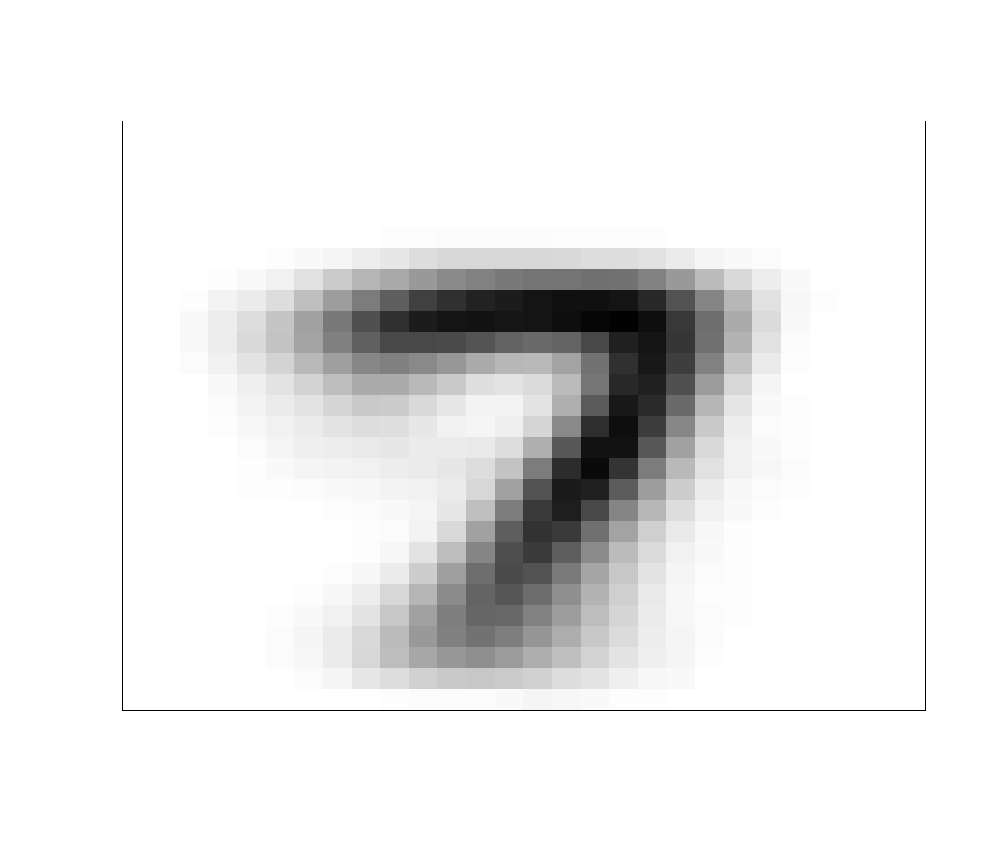
\includegraphics[width=0.5\textwidth]{mu.pdf}
\caption{\label{fig:mu}the mean image of 500 images of the digit ``7\rq\rq{}}
\end{figure}
\begin{figure}

\includegraphics[width=0.8\textwidth]{e-vectors.pdf}
\caption{\label{fig:e-vectors}The 16 first e-vectors for the digit ``7\rq\rq{}}
\end{figure}
\begin{figure}
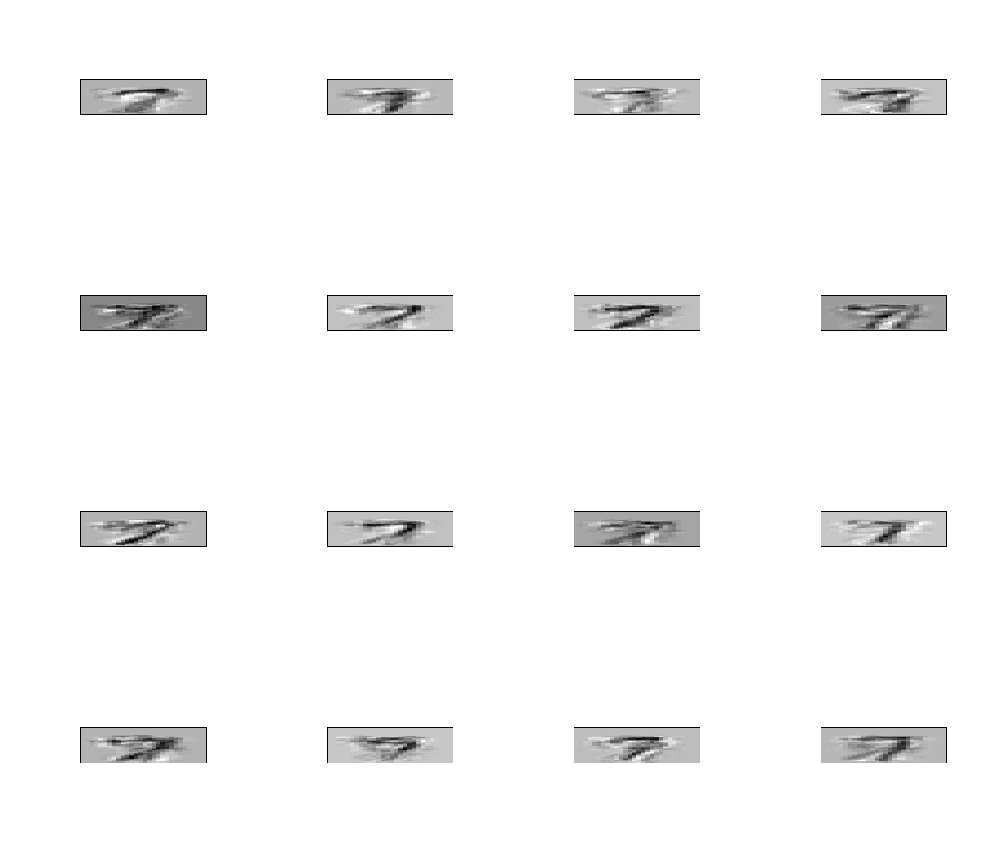
\includegraphics[width=0.8\textwidth]{samples-of-7.pdf}
\caption{\label{fig:samples}16 samples for the digit ``7\rq\rq{}}
\end{figure}
\end{enumerate}
\section{Multiple measurements}
$X \in \mathbb{R}$. $X \sim N(\mu_x,\lambda_0^{-1})$. $Y_1,\ldots,Y_n \in \mathbb{R}$, independent, same distribution $N(x,\lambda^{-1})$ given $x$. Consider observations $y_1,\ldots,y_n$ of $Y_1,\ldots,Y_n$.   
\begin{enumerate}
\item Compute $E[X|y_1,\ldots,y_n]$
\item Compute $Var[X|y_1,\ldots,y_n]$
\end{enumerate}
Note: we have started this exercise in class.
\section{Brownian Bridge}
Let $W_t, t \geq 0$ be a Brownian motion process. That is 
\begin{enumerate}
\item[1)] $W_t, t\geq 0$ is a Gaussian process (GP)
\item[2)] $W_0=0$
\item[3)] $E[W_t]=0, t \geq 0$
\item[4)] $Cov[X_s,X_t]=\min(s,t), s \geq 0, t \geq 0$
\end{enumerate}
Consider the process $B_t$, the Brownian bridge, defined over the interval $0 \leq t \leq 1$ which has the distribution of $W_t$ conditioned on the event $\{W_1=w_1\}$. $B_t$ is a Gaussian process. Compute
\begin{enumerate}
\item$ E[B_t], 0 \leq t \leq 1$
\item $Cov[B_s,B_t], 0 \leq s,t \leq 1$

Hint: Consider an arbitrary collection of time points $t^*=0 \leq t_1^*,\ldots,t_m^*$ and define the vector $W^*=(W_{t_1^*},\ldots,W_{t_m^*})^T$. Then $W^*,W_1$ are jointly Multivariate Normal. Use the usual formula to compute the mean and covariance  of $W^*$ given $\{W_1=w_1\}$. 

\item Take the case $w_1=0$. Propose an algorithm to sample from the Brownian bridge. code it. Plot 3 samples. 
An example is shown in figure \ref{fig:GB}. 
\begin{figure}
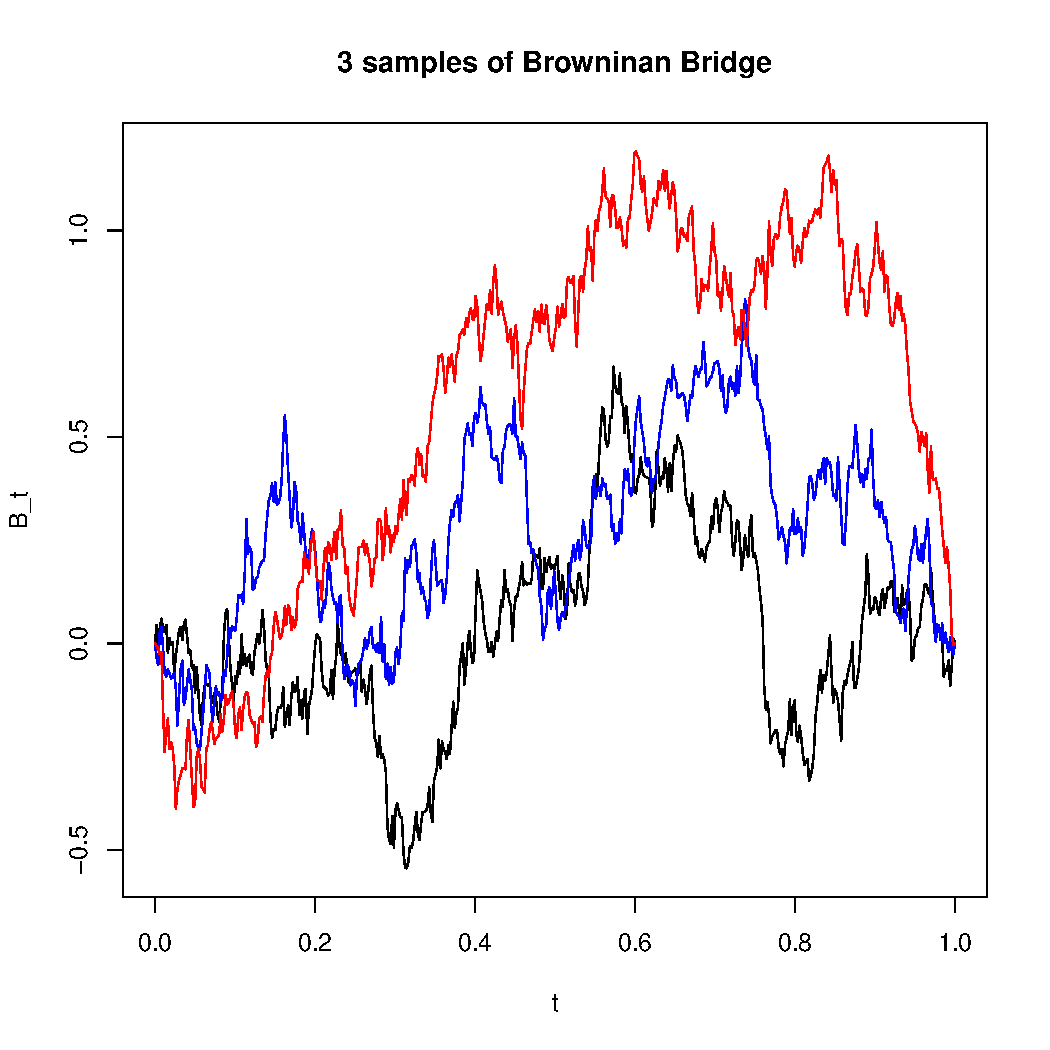
\includegraphics[width=0.5\textwidth]{BB.pdf}
\caption{\label{fig:GB}Samples from the Gaussian Bridge}
\end{figure}
 
\end{enumerate}
\section{Gaussian process with a linear prior}
Consider the following model. $x \in \mathbb{R}$, $k(.,.)$ is a p.d. kernel. $\beta=(\beta_1,\beta_2)^T$ is bivariate random vector.   
\begin{eqnarray}
f & \sim & GP(0,k)\\
\epsilon & \sim & GP(0,\delta) \\
\beta & \sim & N(b,\Sigma) \\
h(x) & = & (1,x)^T\\
g(x) & = & h(x)^T \beta + f(x)\\
y(x) &=& g(x) + \epsilon(x) 
\end{eqnarray}
Moreover, assume that $(f,\epsilon,\beta)$ are independent. Consider a vector of observations $y=(y_1,\ldots,y_n)$ 
\begin{enumerate}
\item Compute $E[\beta|y]$
\item Compute $Cov[\beta|y]$

Hint: write the joint distribution of $(\beta,y)$ then use the usual formula.

Consider now a new point $x^*$,
\item Compute $E[y(x^*)|y]$
\item Compute $V[y(x^*)|y]$

\end{enumerate}

\end{document}
